\documentclass[10pt]{article}
\usepackage{graphicx}

\begin{document}

\title{Free Electron Tutorial for LMPG}
\author{Derek Stewart \\ Cornell Nanoscale Facility \\ Ithaca, NY \\ stewart@cnf.cornell.edu}
\maketitle

\section{Transmission Basics}

In the lmpg code, transport is calculated based on a layered Green's function approach which describes the system in the linear muffin tin orbital (LMTO) framework.  Transmission through the system is found by first determining the Green's function matrix for the device region and then calculating the coupling to the external leads.  The ballistic transmission in this case is given by:

\begin{equation}
T=Tr\left(\Gamma_{11}G^{R}_{1N}\Gamma_{NN}G^{A}_{N1}\right)
\end{equation}
where $G^{R,A}$ are the retarded and advanced Green's functions connecting the ends of the device region.  The $\Gamma$ terms describe how electrons in the device couple to the external leads and can be expressed in terms of the left and right surface Green's functions.  The trace in the expression above is over the available states in the principal layer.

\section{The CTRL file}

We start with a simple test case, the free electron potential step.  The necessary information for this run is contained in the file \textit{ctrl.step} and an atom file \textit{xa.step}.  The \textit{ctrl.step} is the main source of input for lmpg.  This information is divided up by keywords in the ctrl file.  Many of these keywords can be used in general for all of the LMTO codes, however some are specific for the 2D layers case we will be examining.  Information for many of these keywords can be found in the doc section provided with the LMTO code.

In the case of transport, we are interested primarily in the principal Green function or PGF flag.  This tells the code what to do specifically for 2D systems.  This flag is listed first in the ctrl file, \textit{ctrl.step}.  For this flag, various options such as MODE, SPARSE, GFOPTS, etc... are listed.  For now, we will concern ourselves only with the option MODE.  MODE tells the program lmpg whether to run a self-consistent calculation (MODE=1) to determine the proper electronic structure for the interface region or whether to run in MODE=5 to calculate transport properties.  Since we are dealing with a free electron system, we do not need to worry about achieving self-consistency.  Currently the MODE is set to the variable pgf, which is one line above and given by pgf=5.  Lines with a percent sign in front are used to denote external variables.  These terms can be changed at run time so the number of k-points, PGF mode, and other things can be altered quickly.

The next flag of immediate importance is BZ, which stands for Brillioun zone.  This flag determines how many divisions of k points will be done in the BZ for the three directions (NKABC = nkx nky nkz).  In the PGF calculations, we deal with a 2D Brillioun zone, so nkz is set to 1.  In this run, the external variable nk1 sets the number of divisions in $k_{x}$ and $k_{y}$ equal to 4.  The energy range of the calculation is also described in this system.  The nature of the energy calculation and the integration technique is specified by the EMESH parameter.  The EMESH parameter has the following format

\begin{center}
EMESH = n-points mode e-start e-end [other arguments]
\end{center}
where n-points gives the number of energy points on the contour.  The EMESH mode describes what type of energy contour we use.  For self-consistent claculations where the determination of the DOS is crucial, it is much faster to use an energy contour that sweeps out into the complex plane (EMESH mode = 10).  E-start and e-end describe the beginning and end points on the energy contour.  For EMESH mode = 10, there are two more arguments, $ecc$ and $eps$.  The argument $ecc$ determines the eccentricity of the complex contour.  This can range from 0 for a circle, 0.5 for an ellipse, to 1 for a line.  The parameter $eps$ is a bunching parameter which denotes how many sampling points are clustered near the Fermi energy (usually $eps$=0 is fine).  

For transport calculations, we are calculating a quantity that is only analytic on the real axis, \textit{i.e.} the transmission coefficient.  In this case, we must use an energy contour that stays as close to the real axis as possible.  Energy contours that skim the real axis are given by EMESH MODE=1.  In this case, we need one additional argument, \textit{imag-e}, that describes the imaginary part of the energy used for the calculations.  Values on the order of $10^{-5}$ are usually sufficient.  For the free electron case, we are only interested in the transmission, so we use the real axis energy contour.

Next the types of atoms and their positions are given by the flags SPEC and SITE.  The SPEC flag provides information on the atom label and the atom type, XA, with $Z=0$.  This is just an empty sphere used to represent empty space.  The SITE flag lists the position of each atom in the layered structure in terms of x,y,z coordinates and the principal layer index.  In this system, we have a total of 9 principal layers.

Finally, the START flag can be used to determine the number of iterations for a self-consistent claculation (NIT=1) and the level of RMS convergence necessary to stop the program (CNVG=10$^{-6}$).  It can also be used to provide information on individual atoms.  In the free electron case, we specify individual potential values for each atom.  Here we have a potential step (V=0.1) which is 4 principal layers thick. The potential specified can be easily adjusted to match several free electron profiles.

\section{Running the program}

Assuming the lm programs have compiled successfully, we can now start to calculate transmission through systems.  For almost every input file used in the lm family, the structural information of the system must first be prepped by the \textit{lmstr} program.  In lm runs, we only need to use the suffix of the ctrl filename to run programs.

\begin{center}
lmstr step
\end{center}

This program will send out a flurry of date to the screen and then generate two structure files associated with the ctrl file.  Once this is completed, we can run lmpg and calculate the transmission through the system.

To do this, we will use the \textit{lmpg} program which should be in the main directory of your lm distribution.  Type the following:

\begin{center}
lmpg -vnit=1 -vnk1=4 -vpgf=5 step $>$ step.out \&
\end{center}

The dashed terms with the letter \textit{v} stand for variables that can be set at run time.  The variables listed in the command line are $nit$ for the number of iterations, $nk1$ for the number of divisions in the kx and ky BZ directions and pgf for the PGF mode.  All of these variables have a default definition in the file.  I have listed them here to give you practice with the variable option.  For this run, all program output will be sent to a file called \textit{step.out}.  The program could take a few minutes to run.  The left and right surface Green's functions are calculated first for necessary energies and then stored in files for easy access.  For large systems, this portion can take some time and generate large files.  Once lmpg is done, we can grab information about the total transmission and the transmission in different channels.

The transmission will be calculated at three different $k_{||}$ points for a range of energies.  The lmpg code produces two output files which contain the relevant information about transmission for the system under study.  The file jz.step contains a list of different energies, the spin channel, and the real and imaginary parts of the total transmission in column format.

The file jzk.step breaks down the transmission at each energy into contributions from the different $k_{||}$ points.  The first column gives the energy.  The second column indicates the k point index and the third and fourth columns show the real and imaginary parts of the transmission.  If you would like to find out the specific k-point that goes with each k-point index, set PUTQP=t in the BZ section of the CTRL file.  This will print out a qpts file that contains all the k-points used in the calculation along with their associated weights.

Let's look just at the contribution to transmission for electrons with $k_{||}=0$.  These electrons have k index 1.  We can collect them into a seperate file by using the grep command.

\begin{center}
grep ' 1 ' jzk.step $>$ jzk.1.step
\end{center}

Using gnuplot, you can plot out the transmission as follows:

\begin{center} 
gnuplot prompt$>$ plot 'jzk.1.step' using 1:3
\end{center}
or if you want the energy in eV...

\begin{center}
gnuplot prompt$>$ plot 'jzk.1.step' using (13.6*\$1):3
\end{center}

You will see basically no transmission for electron energies lower than the potential barrier.  Once the energy of the electron is greater than the potential barrier, there are some oscillations in the transmission around 1 that are related to the quantum nature of the interaction.  These oscillations are well described in standard quantum physics books.  The oscillations can be described analytically and are related to the step height and step width.  The transmission for the first ($\Gamma$) k-point and the second k-point are shown in Figure ~\ref{jzk.1and2.step}.  When you plot the transmission for the second and third k-points, the jump up in transmission will be higher in energy.  This is due to the fact that the electron is striking the potential barrier at a glancing angle.  Therefore all of the electron energy is not in the $z$ direction.  For the first k point, the electron strikes at normal incidence to the potential barrier, so all the energy is in the $z$ direction.  For the 2nd and 3rd k-points, since only a fraction of the total energy is used to propogate in the z direction, a higher total energy is required to transmit across the potential barrier.

\begin{figure}
\begin{center}
\centering
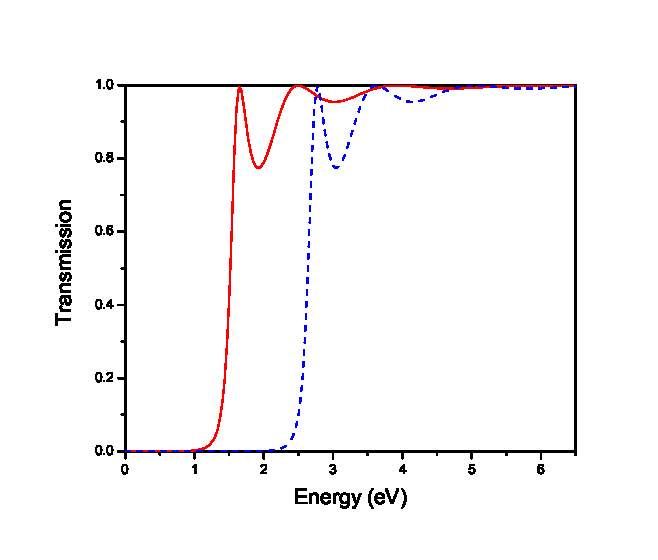
\includegraphics[angle=0,width=9.00cm]{jzk.1and2.step.eps}
\caption{Transmission across the potential step for the $\Gamma$ k-point (red line) and k-point (0.25,0,0) in the blue dashed line.}
\label{jzk.1and2.step} 
\end{center}
\end{figure}


We can also examine the total transmission across the potential barrier summed over k-points.  To plot the total transmission, use the following gnuplot command:

\begin{center}
gnuplot prompt$>$ plot 'jz.step' using (13.6*$1$):3
\end{center}

This will give a transmission curve which has a series of steps (Fig.~\ref{total_trans_step}).  Each step corresponds to the energy where an additional electron with a different k point is able to transmit over the barrier.  You should be able to compare the individual transmission results for the different jzk and see a similar shift in transmission.

\begin{figure}
\begin{center}
\centering
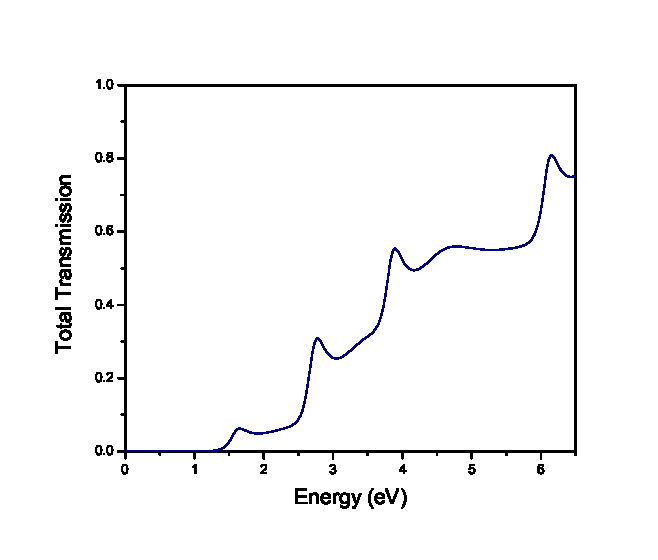
\includegraphics[angle=0,width=9.00cm]{step_transmission.eps}
\caption{Total transmission across a potential step.  The transmission profile has a series of humps that can be related to quantum interference when an electron at a given k point has nearly the same energy in the $z$ direction as the potential barrier.}
\label{total_trans_step} 
\end{center}
\end{figure}


\section{Adjusting the Free Electron Potential}

To change the potential the free electron experiences, you will need to adjust the potentials given to the atoms below the START command in the ctrl.step file.  Don't forget that the potentials are given in units of Rydbergs.

\begin{verbatim}
START   NIT=1 FREE=F BEGMOM=F CNTROL=T CNVG=1D-6 RDVES=T
        ATOM=XA   V={0}
        ATOM=XA2 V={0}
        ATOM=XA3 V={0}
        ATOM=XA4  V={0}
        ATOM=XA5 V={0}
        ATOM=XA6  V={0}
        ATOM=XA7 V={0.1}
        ATOM=XA8 V={0.1}
        ATOM=XA9 V={0.1}
        ATOM=XA10 V={0.1}
        ATOM=XA11 V={0.1}
        ATOM=XA12 V={0.1}
        ATOM=XA13 V={0.1}
        ATOM=XA14 V={0.1}
        ATOM=XA15 V={0}
        ATOM=XA16 V={0}
        ATOM=XA17 V={0}
        ATOM=XA18 V={0}
        ATOM=XA19 V={0}
        ATOM=XA20 V={0}
        ATOM=XA21 V={0}
        ATOM=XA22 V={0}
\end{verbatim}

Beside each atom a potential is specified.  To increase the potential step, just change V=0.1 to something like 0.3.  To increase the width of the potential step, just increase the number of atoms with a potential shift.  In the next section, I will show you how you can adjust the potential profile to consider a free electron model for a leaky quantum well.

\section{Quantum Well Model}

We can think of a quantum well as a layered system consisting of a central region and two high potential barriers on either side that confine electrons in the system.  Since the barriers are not infinite, there should still be some coupling between the quantum well and the leads outside.  In fact, for certain incident electron energies, the electrons are resonant with the quantum well states.  This leads to near perfect transmission through the system for very narrow energy ranges.  In this manner, the transmission can be used to probe the quantum well energy states and also to see how well it couples to the external leads.  

We can set up this system by adjusting the potential profile provided in the ctrl.step file.  First make a new directory and copy ctrl.step into that directory.  Then rename ctrl.step to ctrl.well.  Just as we did in the step case, we will need to generate the appropriate structure files using the lmstr program.  Now edit the ctrl.well file so that the potential profile looks like the one given below.

\begin{verbatim}
START   NIT=1 FREE=F BEGMOM=F CNTROL=T CNVG=1D-6 RDVES=T
        ATOM=XA   V={0}
        ATOM=XA2 V={0}
        ATOM=XA3 V={0}
        ATOM=XA4  V={0.4}
        ATOM=XA5 V={0.4}
        ATOM=XA6  V={0.0}
        ATOM=XA7 V={0.0}
        ATOM=XA8 V={0.0}
        ATOM=XA9 V={0.0}
        ATOM=XA10 V={0.0}
        ATOM=XA11 V={0.0}
        ATOM=XA12 V={0.0}
        ATOM=XA13 V={0.0}
        ATOM=XA14 V={0.0}
        ATOM=XA15 V={0.4}
        ATOM=XA16 V={0.4}
        ATOM=XA17 V={0}
        ATOM=XA18 V={0}
        ATOM=XA19 V={0}
        ATOM=XA20 V={0}
        ATOM=XA21 V={0}
        ATOM=XA22 V={0}
\end{verbatim}

Also, please make sure to copy over the atom file xa.step and rename it xa.well.  We can now run lmpg to calculate the transmission through the system.  We use the same command as before:

\begin{center}
lmpg -vnit=1 -vpgf=5 -vnk1=4 well $>$ out.well \&
\end{center}

Now we can examine the jz.well file with contains the total transmission.  If we plot this (Fig. ~\ref{total_trans_well}), we see quite a different transmission profile from the potential step we considered earlier.  Now the transmission is made up of a series of sharp peaks that correspond to resonances with the quantum well energy levels.  It is also clear that the broadening associated with the peaks varies.  This is due to how well the quantum well couples with the external leads.  Greater broadening of the peak indicates more leakage from the quantum well.  

\begin{figure}
\begin{center}
\centering
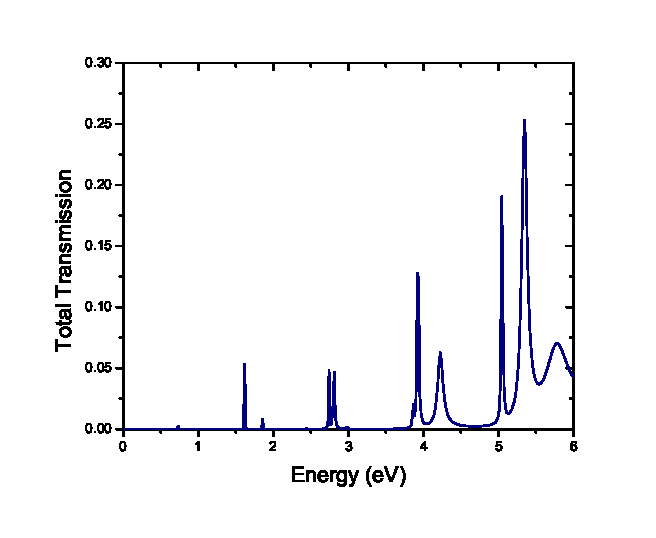
\includegraphics[angle=0,width=9.00cm]{well_transmission.eps}
\caption{Total transmission across a quantum well.  Notice that the resonant transmission peaks have different degrees of broadening.  This is related to how well they couple to the external leads.}
\label{total_trans_well} 
\end{center}
\end{figure}

The total transmission sums over all the k points considered and this leads to a overlap of different resonant profiles that occur at different k points.  We can isolate the transmission profile from different k points by grepping out the transmission contributions from the jzk.well file.  The transmission profiles for the first and second k-points are shown in Figure ~\ref{k_trans_well}.  For the first k point, the electron is directly incident on the quantum well barriers and this results in it being resonant with the quantum well states at lower energies than electrons that hit the barrier at an oblique angle.  Notice that the resonant states for the second k-point start at higher energy.  This is similar to what we observed with the potential step earlier.

\begin{figure}
\begin{center}
\centering
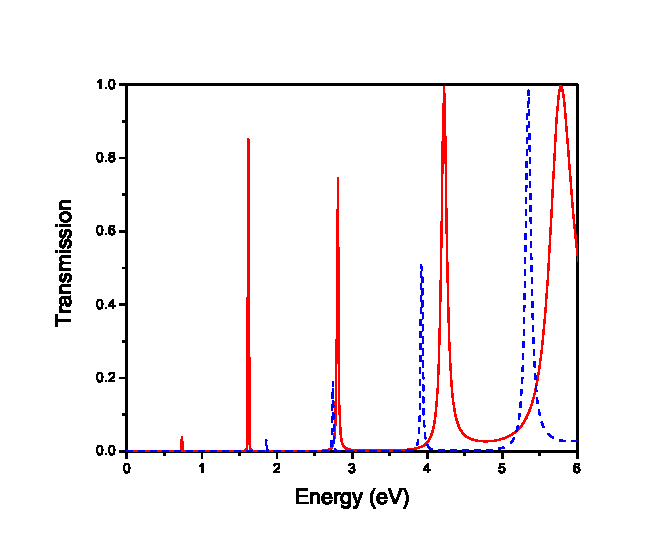
\includegraphics[angle=0,width=9.00cm]{jzk.1and2.well.eps}
\caption{Transmission across a quantum well for two different k points, $\Gamma$ (red line) and for k-point (0.25,0,0) in the blue dashed line.}
\label{k_trans_well} 
\end{center}
\end{figure}

\section{Where to Go from Here}
I hope this free electron tutorial has given you some idea of the power of the lmpg code.  Using even these simple models, we can develop insight into devices that are at the forefront of research today, such as resonant tunneling devices and tunneling barrier systems.  Please refer to the following articles below for more information.\\

\noindent S. Faleev, F. Leonard, D. A. Stewart, and M. van Schilfgaarde, "\textit{Ab-initio} TB-LMTO method for non-equilibrium electron transport in nanosystems", \textit{Physical Review B}, \textbf{71}, 195422, (2005). \\

\noindent K. D. Belashchenko, E. Y. Tsymbal, M. van Schilfgaarde, D. A. Stewart, I.I. Oleinik, and S. Jaswal, "Effect of Interface Bonding on Spin-Dependent Tunneling from oxidized Co Surfaces", \textit{Physical Review B}, \textbf{69}, 174408, (2004). \\

\noindent D. A. Stewart and M. van Schilfgaarde, "Digitally doped magnetic resonant tunneling devices: High tunneling magnetoresistance systems", \textit{Journal of Applied Physics}, \textbf{93}, 7355, (2003).

\section{Contact Info}
For more information or to report bugs, please contact Derek Stewart at stewart@cnf.cornell.edu.  

 


\end{document}
